\chapter{Implementation}

It would be very difficult to attempt to build a complete working system
during the course of the project, and that would be wholly out of scope. So
throughout this project, the idea has been to build prototypes that
demonstrate that a fully production-ready solution is viable.

A lot of the development work was also slowed down by a number of unforseen
hardware issues, which are detailed in this chapter along with other
implementation details.

\section{Developing The Base Station Code}
The main base station program is just a \acrshort{tcp} server that handles
commands coming in from the camera and motion sensors over the \gls{6lowpan}
connection. Since the Linux kernel can already handle the \gls{6lowpan}
connection, and no other hardware interfaces are required, there was a lot of
flexibility in the choice of language and framework used to build the server.
The Python language ended up being the choice of language, for its ease of
development and pseudocode-like syntax.

The core language library also includes the \texttt{socket} library, which
provides an easy to use, low-level interface for opening and accepting UDP
and \acrshort{tcp} connections. The server has a global dictionary that maps
the id numbers of sensor pairs to the id of a camera sensor and the id of a
motion sensor. This dictionary is populated from sensors which send an
identification (\texttt{id}) command, broadcasting their unique
\texttt{sensor\_id} and their \texttt{pair\_id}. This means that, when a
motion sensor sends a motion detection command to the server, the server can
look up the ID of the camera associated with the motion sensor and send it a
command to capture a photo.

The source code for the base station server is available in section
\ref{code:base-main} \textit{(page \pageref{code:base-main})}.

\subsection{Developing The Species Classifier}
Less time was available in practice for developing the species classification
software than intended, because of the complications arising from developing
for the remote sensors as well trying to use the camera module. However, some
exploration was made into the the techniques available to detect and classify
species from a photo image.

Naturally, this was a problem well suited for a \acrfull{cnn}.
\acrshort{cnn}s, according to Christopher Olah's blog post on the
subject~\cite{olah2014conv}, ``can be thought of as a kind of neural network
that uses many identical copies of the same neuron''. Each of these `neurons'
uses contains a mathematically trivial function, such as calculating mean
averages of a set of pixel colours, to reduce the problem down. Weighted
values are used to interpret these outputs and produce the final output of
the network. These weights are ``trained'' (adjusted) using a training set of
data, so that the network's output matches the expected output.

Because of the unforseen issues surrounding the \gls{6lowpan} connectivity
and the camera sensor, there was less time than planned to develop a
prototype classification program. However, some exploration was made into the
techniques that could be used to build a classifier that can run on the Ci40
board.

\subsubsection{Defining A Model}
The first step to defining a deep learning model is to specify the input and
the output. The input is a 172 by 144 pixel (also known as ``QCIF format'')
image captured using the camera sensor, while the output is a probability
distribution of size $N$, giving the probabilities that the content of the
image is one of $N$ different categories\textemdash{}in this case, it would
be the list of animals we are classifying for, as well as a ``no animal''
category and a ``unknown'' category. And as for the intermediary steps in the
model? That's where a trained \acrlong{cnn} is used.

\acrshort{cnn}s are made up of a set of ``layers'', which are put together to
form the network. According to the Stanford CS231n course
notes~\cite{cs321n-cnn}, there are five main types of layers:

\begin{itemize}
  \item Input layer\textemdash{}the raw data input into the network. For this
  project, the 172x144 pixel images from the camera sensor.
  \item Convolutional layer\textemdash{}a layer of neurons that each perform
  a compution on a small region, or a ``kernel'', of the image. Multiple
  ``filters'' may be used in this layer to detect different features. E.g.
  one filter may detect vertical edges, another may detect horizontal edges.
  \item Activation layer\textemdash{}applies some kind of activation function
  to each output from the previous layer to determine whether the neuron
  ``fires'' or not. The simplest example, also given by the CS231n course
  notes~\cite{cs321n-cnn} is a threshold function like $max(0, x)$, which
  will have a range of $\{ 0, \mathbb{N}^{+} \}$.
  \item Pooling layer\textemdash{}Performs operations on groups of neurons to
  result in a smaller output. Useful for working on large, high-level
  features in images.
  \item Fully-connected layer\textemdash{}this is the final layer in the
  network, and takes \textit{all} outputs from the previous layer and creates
  the final output; in this case it will produce a list of probabilities of
  the image being classified into a certain category/species.
\end{itemize}

% thanks to https://github.com/jettan/tikz_cnn
%
%
\begin{figure}
	% \noindent\resizebox{\textwidth}{!}{
  \centering
	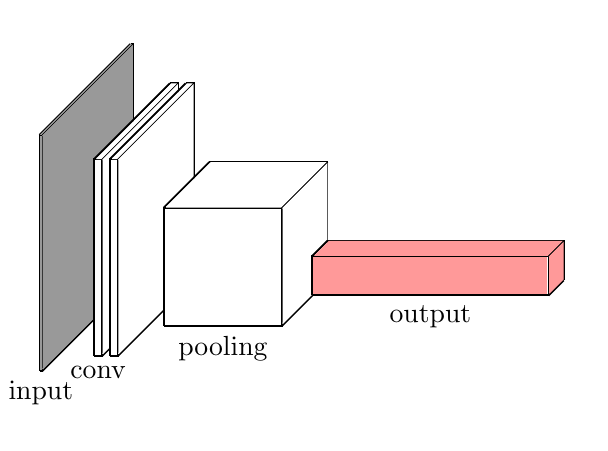
\begin{tikzpicture}
		\draw[use as bounding box, transparent] (-1.8,-1.8) rectangle (5.2, 3.2);

		% Define the macro.
		% 1st argument: Height and width of the layer rectangle slice.
		% 2nd argument: Depth of the layer slice
		% 3rd argument: X Offset --> use it to offset layers from previously drawn layers.
		% 4th argument: Options for filldraw.
		% 5th argument: Text to be placed below this layer.
		% 6th argument: Y Offset --> Use it when an output needs to be fed to multiple layers that are on the same X offset.

		\newcommand{\networkLayer}[6]{
			\def\a{#1} % Used to distinguish input resolution for current layer.
			\def\b{0.02}
			\def\c{#2} % Width of the cube to distinguish number of input channels for current layer.
			\def\t{#3} % X offset for current layer.
			\ifthenelse {\equal{#6} {}} {\def\y{0}} {\def\y{#6}} % Y offset for current layer.

			% Draw the layer body.
			\draw[line width=0.25mm](\c+\t,0,0) -- (\c+\t,\a,0) -- (\t,\a,0);                                                      % back plane
			\draw[line width=0.25mm](\t,0,\a) -- (\c+\t,0,\a) node[midway,below] {#5} -- (\c+\t,\a,\a) -- (\t,\a,\a) -- (\t,0,\a); % front plane
			\draw[line width=0.25mm](\c+\t,0,0) -- (\c+\t,0,\a);
			\draw[line width=0.25mm](\c+\t,\a,0) -- (\c+\t,\a,\a);
			\draw[line width=0.25mm](\t,\a,0) -- (\t,\a,\a);

			% Recolor visible surfaces
			\filldraw[#4] (\t+\b,\b,\a) -- (\c+\t-\b,\b,\a) -- (\c+\t-\b,\a-\b,\a) -- (\t+\b,\a-\b,\a) -- (\t+\b,\b,\a); % front plane
			\filldraw[#4] (\t+\b,\a,\a-\b) -- (\c+\t-\b,\a,\a-\b) -- (\c+\t-\b,\a,\b) -- (\t+\b,\a,\b);

			% Colored slice.
			\ifthenelse {\equal{#4} {}}
			{} % Do not draw colored slice if #4 is blank.
			{\filldraw[#4] (\c+\t,\b,\a-\b) -- (\c+\t,\b,\b) -- (\c+\t,\a-\b,\b) -- (\c+\t,\a-\b,\a-\b);} % Else, draw a colored slice.
		}

		\networkLayer{3.0}{0.03}{-0.5}{color=gray!80}{input}

		\networkLayer{2.5}{0.1}{0.0}{color=white}{conv}{}    % S1
    \networkLayer{2.5}{0.1}{0.2}{color=white}{}{}        % S2
    
    \networkLayer{1.5}{1.5}{0.5}{color=white}{pooling}{}

		% OUTPUT
		\networkLayer{0.5}{3.0}{2.0}{color=red!40}{output}{}          % Pixelwise segmentation with classes.


	\end{tikzpicture}
	% }
 \caption{A visualisation of how the convolutional neural network would have
 been structured, with each image inputted as a square image with red, green,
 and blue colour channels; the one or more convolutional layers which filter
 for local features; a pooling layer which groups together low-level features
 to find high-level image patterns; and finally an output layer which ouputs
 a one-dimensional list of probabilities for each animal species.}
	\label{fig:cnn}
\end{figure}

Figure~\ref{fig:cnn} shows a visualisation of how the layers of our neural
network would interact with each other. Three-dimensional space is required
since each layer is three-dimensional; the input, for example, takes an image
with a width, height and three colour values for each pixel.

\subsubsection{Finding A Suitable Training Set}

Manually building and labelling a set of images to train the model would have
taken an extremely long time, since thousands of images would have to be
obtained to help prevent the model from being \gls{overfit}ted to the training
data (although other methods such as using the ``Dropout''
technique~\cite{srivastava2014dropout} can also reduce overfitting). For a
production-ready system, a bespoke training set would be very suitable,
especially for longer-term projects. However, for this prototype system, it
was decided to use a pre-existing training set to focus purely on the deep
learning model.

The first choice was to find a training set with woodland animals, which
would be pertinent to this project. Unfortunately none were found, so the
next best fit would be any kind of annotated camera trap data. Fortunately, a
set of over four thousand camera annotated trap images, classified by
``multiple experts'', was published as part of the Snapshot Serengeti
project~\cite{swanson2015snapshot} and released
online~\cite{swanson2015data}. The images are annotated with the number of
species in the image, an id relating to one of 48 species in the dataset (or
``unknown''), and the number of individual animals in the image.

Although this training data is not \textit{exactly} the kind of data that
would be collected in a production-ready version of this project, it provides
a good enough picture of the kinds of challenges that may be faced by such a
deep learning model in this project's application, such as views being
obstructed by foliage, multiple species being visible, and images where it is
impossible to determine what species is in the photo.

The script detailed in Section~\ref{code:classify-getimages} is used to
download the Project Serengeti gold standard data set file (formatted as a
\acrshort{csv} file), as well as the \acrshort{csv} file containing the URL
of each image by ID. It then filters the list for the training set we want
(images with only a single animal in the photo), fetches the actual photo,
then resizes it into a common format (128x128 pixel JPEG file). This results
in 1572 images to be used for testing and training. The test data is split,
so that roughly the first eight percent (1250) of the images are used for
training, and roughly the last twenty percent (322) are used for testing the
model. A nice round number for the training set size is helpful so that the
training can occur in batches.

\subsubsection{Architectural Incompatibilities}
The biggest drawback to using TensorFlow to develop an image classifier is
that it only supports 64-bit architectures~\cite{tensorflow-sysreq}.
Therefore, it will not run as-is on a 32-bit processor, such as the one that
the Ci40 uses. However, methods exist to generate a 32-bit model from a
standard TensorFlow model exist, and are provided by the project itself. Arm,
the mobile chip designer and manufacturer, provide a detailed tutorial for
achieving this~\cite{arm-tensorflow32bit}. Theoretically it would then be
possible to use this compiled 32-bit TensorFlow model onboard the Ci40 device
for embedded classifier operations.

Another possible solution would have been to use an alternative deep learning
framework. Other possibilities included using the Caffe deep learning
framework~\cite{jia2014caffe}, or a high-level framework like
Keras~\cite{keras}. However, the overwhelming amount of tutorials and
documentation for TensorFlow available on the Internet meant that it was
still a sensible choice of framework.

\section{Developing The Remote Sensor Code}
The \gls{6lowpan} clicker that the motion and camera sensors use runs on a
\acrfull{rtos} called \textit{Contiki}~\cite{contiki}. The code that runs on
these devices has to be flashed to the onboard flash memory. Therefore,
Creator provide their own toolchain for compiling and flashing user code.
This, however, was extremely difficult to set up, and a lot of time was spent
obtaining the tooling, attempting to install the code, and being able to
access the clicker from my computers. A lot of documentation was missing or
not provided, which made independent investigations into the source code
necessary.

Another issue was with writing the sensor code itself. The only provided
documentation for Contiki is a handful of examples on its source code
repository, as well as a tutorial on the Creator
website~\cite{clickersetupguide}. To complicate matters further, the code
used to program the boards is a modified version of the C language, except
code runs in ``process threads''. However, after a lot of searching on the
web, the Contiki wiki was discovered~\cite{contiki-wiki}. Despite being
incredibly technical, there was helpful pieces of information available there
to help decipher the inner workings of the Contiki platform, notably how the
``protothreads'' work.

Debugging the code was a further complication when developing the sensor
code. The \gls{6lowpan} clicker only has a single MicroUSB port, which is
used for flashing code to the onboard memory, and does not have a USB port of
any kind to connect a serial terminal to. There is only two ways of debugging
the clicker\textemdash{}sending text over the \gls{6lowpan} connection, or
setting the two hardware LEDs on or off. A \acrshort{udp}-based debugging
server is available along with a \texttt{PRINTF} macro, however these did not
appear to work very well, if at all. It was also found that the debugging
server would not work if the device was making a separate connection to the
base station, such as when sending motion commands.

\subsection{6LoWPAN issues}
A reoccurring issue throughout the development of the remote sensors was the
reliability of the \gls{6lowpan} connection. It often took multiple minutes
or more for the remote sensors to connect to the base station, regardless of
whether it was a \acrshort{tcp} connection or a \acrshort{udp} connection.
Sometimes, the devices would not connect at all, and the debugging server
(when it worked) reported multiple dropped messages. Since the Ci40 uses the
2.4 \acrshort{ghz} frequency band, which is shared with many WiFi standards
as well as Bluetooth, there is a possibility that this might be caused by
interference between these devices, especially since all of the testing
environments available during this project were in close proximity to WiFi
links as well as Bluetooth devices, despite best efforts.

A manual published by \textit{NXP Semiconductors} highlights the issues that
can occur from the co-existence of these technologies on the same 2.4
\acrshort{ghz} frequency band~\cite{nxp2013ieee802154coexistence}. Notably,
on page 19, they recommend that ``to achieve satisfactory IEEE 802.15.4
[6LoWPAN] performance in the presence of WLAN interference, a channel
centre-frequency offset of 7 MHz is recommended'', and if \gls{6lowpan} is
running on the same channel as the WiFi link, ``a physical separation from
the WLAN \acrfull{ap} of 8 m is recommended''. Essentially, they recommend
either conducting radio operations away from WiFi \acrshort{ap}, or selecting
a different channel if possible. However, the WiFi \acrshort{ap}s in the
testing environment are managed by a third party, so it was not possible to
change their channels. Additionally, the documentation for the Ci40 base
station was not clear enough on whether it was possible to set the
\gls{6lowpan} wireless channel or not.

As a result of these \gls{6lowpan} issues, some modifications were made to
the project. The camera sensor would be prototyped by installing the camera
module \textit{directly} onto the Ci40 base station, to make development and
debugging easier. Since the Ci40 runs a full Linux operating system and full
WiFi stack, it is possible to connect to it using an \acrfull{ssh}
connection. In addition to this, code designed to run on the camera clicker
was not developed because it would be extremely similar to the motion sensor
code, albeit with the camera processing code instead of the motion sensor
event handling code.

\subsection{Working With The Camera Click Module}
One of the biggest obstacles during the project was working with the
\textit{MikroElektronika Camera Click} module~\cite{cameraclick}, to be used
as part of the prototype hardware for the remote camera sensor. The only
documentation provided for this sensor is available on their ``LibStock''
website~\cite{cameraclickexamples}, but the only documentation provided is a
board schematic and a code example, designed to be used with
\textit{MikroElektronika}'s own TFT display, with its own proprietary image
format.

However, the code example provided was enough to discover roughly how the
camera click board works and responds to input. It uses the \acrshort{spi}
interface to receive commands and send a new or buffered image back to the
parent device. The commands supported are, according to the code examples:

\begin{itemize}
  \item \texttt{\_\_CMD\_WRITE\_REG} (assumed) write to the registers on the
  camera \acrfull{mcu}, to set things like exposure and brightness settings.
  \item \texttt{\_\_CMD\_READ\_REG} (assumed) read from the registers on the
  camera \acrshort{mcu}.
  \item \texttt{\_\_CMD\_GET\_FRAME} capture a new photo and prepare to send
  it back through the \acrshort{spi} interface.
  \item \texttt{\_\_CMD\_GET\_FRAME\_BUFFERED} (assumed) get the currently
  buffered image from the camera, without capturing a new image.
  \item \texttt{\_\_CMD\_SET\_ROW\_NUM} unknown.
  \item \texttt{\_\_CMD\_SET\_ROW\_SIZE} unknown.
\end{itemize}

\subsubsection{The \acrshort{spi} Interface}
The \acrshort{spi} involves one ``master'' device, which sends commands to
one or more ``slave'' devices. There is four data lines involved:

\begin{itemize}
  \item CS\textemdash{}Chip Select. Selects the slave device to use.
  \item MISO\textemdash{}Transmits data from the master device to the slave
  device.
  \item MOSI\textemdash{}Transmits data from the slave device to the master
  device.
  \item CLK\textemdash{}Timing signal.
\end{itemize}

The master and slave devices transmit data as if they were one ``rotary''
system. Each side has a buffer of a fixed size (in the case of the camera
module, 8 bits), and as the master device pushes a bit to the \acrshort{spi}
interface, the slave device sends a bit back. This continues until the
buffers are essentially swapped around (see figure~\ref{fig:spi}). One
peculiarity in this implementation of \acrshort{spi} is that the camera
module use sa separate ``interrupt'' pin (provided by the \gls{mikrobus}
standard) to let the master device know that it is ready for commands.

\begin{figure}[h]
  \centering
  \includegraphics[width=0.8\textwidth]{spi}
  \caption{A diagram showing data being swapped between two SPI devices.
  Image created by Cburnett on Wikimedia Commons. Obtained from Wikimedia
  Commons under the GNU Free Documentation License. Source: 
  \url{https://commons.wikimedia.org/wiki/File:SPI_8-bit_circular_transfer.svg}}
  \label{fig:spi}
\end{figure}

\subsubsection{Getting Camera Output}
The code in Section~\ref{code:camera-base} shows the code used to attempt to
obtain output from the camera sensor, installed onto one of the Ci40's
\gls{mikrobus} ports. It works by initialising the \acrshort{spi} pins and
setting speed and other settings, before waiting for the camera to send a
``ready'' signal and then sending the \acrshort{spi} command to get an image
from the camera. It then reads the incoming data to a buffer, and saves that
buffer to a file. The data \textit{should}, in theory, be the image data from
the camera. This code should work since it roughly follows the steps used in
\textit{MikroElektronika}'s example code. However, the camera module
frequently returns a lot of blank data. Below is one example of data received
from the camera sensor after sending a \texttt{\_\_CMD\_GET\_FRAME} command:

\begin{verbatim}
  [mbell@chancery-lane ~]$ hexdump ~/out.bin
  0000000 ffff ffff ffff ffff ffff ffff ffff ffff
  *
  000c600 0000 0000 0000 0000 c611               
  000c60a
\end{verbatim}

\subsubsection{Interpreting Camera Output}
Sometimes the camera would send data that was not just a stream of \texttt{1}
bits, however it was not clear whether the returned data was nonsense, or if
the data was in some proprietary data format.

Figure~\ref{fig:yuvimage} shows the data previewed as a \textit{YUV} image.
This is an 8-bit pixel encoded image format that contains three values for
each colour\textemdash{}the brightness (also called luminance), and two
values defining the colour itself (the chroma)~\cite{softpixelyuv}. The data
was estimated to be using some kinda of YUV format, because of reoccurring
patterns in the data that suggested that pixel data was set as some 4-bit
value, then two 2-bit values.

The possibility of the data being stored as \acrfull{rgb} data was ruled out
when attempting to parse the raw image file as such. The results can be seen
in figure~\ref{fig:rgbimage}. It is clear that the data is not \acrshort{rgb}
since the rendering software runs out of bits roughly two-thirds of the way
through parsing the image. Since public access to the source code for the
camera module was prohibited by the manufacturer, it was impossible to tell
whether the image format chosen was incorrect, or if the camera module itself
was defective or damaged. Therefore, no image was ever able to be correctly
obtained from the camera module.

\begin{figure}[h]
  \centering
  \includegraphics[width=0.8\textwidth]{cameraoutput1}
  \caption{The data received from the camera sensor, interpreted as a
  YUV-formatted image.}
  \label{fig:yuvimage}
\end{figure}

\begin{figure}[h]
  \centering
  \includegraphics[width=0.8\textwidth]{cameraoutput2}
  \caption{The data received from the camera sensor, interpreted as a
  RGB-formatted raw image.}
  \label{fig:rgbimage}
\end{figure}

\subsubsection{Read-Only Register Random Number Generator}
The camera module used on the camera sensor is the OV7670-VL2A CMOS sensor,
and a datasheet is readily available online~\cite{omnivisiondatasheet}.
Included in the datasheet is a list of the sensor's registers, detailing each
register's:

\begin{itemize}
  \item One-byte address (in hexadecimal),
  \item Name of the register,
  \item The default hexadecimal value,
  \item Whether it can be read and/or written to,
  \item And a description of what the register represents.
\end{itemize}

Two of these registers were of significance for testing the \acrshort{spi}
interface, addresses \texttt{1C} and \texttt{1D}. These are both read-only
registers that return the high byte and low byte (respectively) of the two
byte manufacturer ID. They are both read only and are supposed to always
return \texttt{0x7F} and \texttt{0xA2} respectively.

However, when this was attempted on the \texttt{camera\_base} application
(see Section~\ref{code:camera-base} lines 141\textendash{}144), the program
received random numbers each time (see Figure~\ref{fig:missingmessages} for
server output). Either one of two explanations is possible\textemdash{}either
the code to read from the register is incorrect, or the camera click board is
defective. As with trying to read the image itself, it is impossible to
conclude which of these explanations is correct without being able to access
the \textit{MikroElektronika} source code.

\begin{figure}[h]
  \centering
  \includegraphics[width=0.8\textwidth]{missingmessages}
  \caption{Screenshot of a terminal image showing the debugging server
  missing messages from the remote sensor.}
  \label{fig:missingmessages}
\end{figure}

\section{Developing The API Server}
The \acrshort{api} server was built entirely using the Node.js
framework~\cite{nodejs}, which runs JavaScript code on computers and servers
without a web browser. It was chosen for ease of development, and since the
server would be managing a \acrshort{json} \acrshort{api}, it made sense to
use a language which natively supports \acrshort{json} too.

The server framework used was Koa~\cite{koa}, which supports modern
JavaScript features such as asynchronous functions. Almost all helper
functionality (such as URL routing) is not provided as part of the core
package, meaning that the library has a very small blueprint\textemdash{}this
is very useful for fast deployment to cloud servers. The database of choice
was PostgreSQL; this again was a choice made because of similarity with the
program, as well as very few differences between it and its competition (for
example, MySQL and MariaDB).

All of the code was developed using a \acrfull{bdd} methodology, meaning that
tests were written before the code itself. This is expanded on in more detail
in the \textit{Testing} chapter. The final code can be found in the appendices.